\documentclass[border=2pt]{standalone}
\usepackage[T1]{fontenc}
\usepackage[scaled]{helvet}
\renewcommand{\familydefault}{\sfdefault}
\usepackage{tikz}
\usetikzlibrary{positioning,arrows.meta,calc}
\begin{document}
\footnotesize
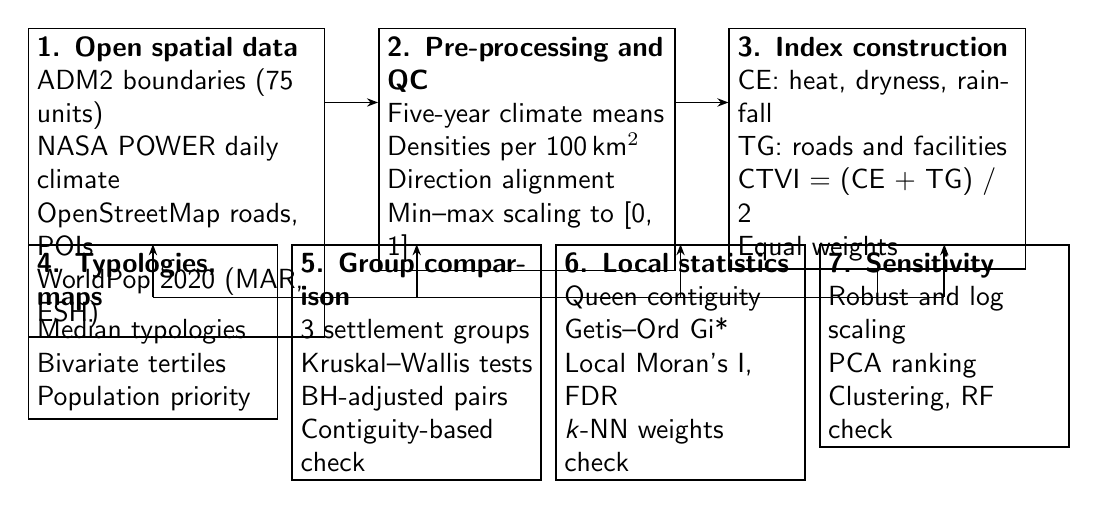
\begin{tikzpicture}[
  box/.style={draw=black, line width=0.6pt, align=left, anchor=north west,
              inner sep=3pt, text width=#1},
  box/.default=3.55cm,
  arr/.style={-{Stealth[length=4pt]}, line width=0.6pt}]
\node[box] (b1) at (0,0) {\textbf{1. Open spatial data}\\ADM2 boundaries (75 units)\\NASA POWER daily climate\\OpenStreetMap roads, POIs\\WorldPop 2020 (MAR, ESH)};
\node[box] (b2) at (4.45,0) {\textbf{2. Pre-processing and QC}\\Five-year climate means\\Densities per 100\,km$^{2}$\\Direction alignment\\Min--max scaling to [0, 1]};
\node[box] (b3) at (8.9,0) {\textbf{3. Index construction}\\CE: heat, dryness, rainfall\\TG: roads and facilities\\CTVI = (CE + TG) / 2\\Equal weights};
\draw[arr] (b1.east |- 0,-0.95) -- (b2.west |- 0,-0.95);
\draw[arr] (b2.east |- 0,-0.95) -- (b3.west |- 0,-0.95);
\node[box=2.95cm] (b4) at (0,-2.75) {\textbf{4. Typologies, maps}\\Median typologies\\Bivariate tertiles\\Population priority};
\node[box=2.95cm] (b5) at (3.35,-2.75) {\textbf{5. Group comparison}\\3 settlement groups\\Kruskal--Wallis tests\\BH-adjusted pairs\\Contiguity-based check};
\node[box=2.95cm] (b6) at (6.7,-2.75) {\textbf{6. Local statistics}\\Queen contiguity\\Getis--Ord Gi*\\Local Moran's I, FDR\\\textit{k}-NN weights check};
\node[box=2.95cm] (b7) at (10.05,-2.75) {\textbf{7. Sensitivity}\\Robust and log scaling\\PCA ranking\\Clustering, RF check};
\coordinate (split) at ($(b3.south)+(0,-0.35)$);
\draw[line width=0.6pt] (b3.south) -- (split);
\draw[line width=0.6pt] (b4.north |- split) -- (b7.north |- split);
\foreach \b in {b4,b5,b6,b7} \draw[arr] (\b.north |- split) -- (\b.north);
\end{tikzpicture}
\end{document}
